\chapter{Introduction}
% Tot mai multe persoane au nevoie de recuperare medicala din toate categoriile de varsta.  
% Exista multe cazuri in care apare un o problema medicala care poate fi rezolvata prin recuperare.

More and more people need medical recovery from all age groups.
There are many cases where there is a medical problem that can be resolved by medical recovery.

% De exemplu in cazul persoanelor care sufera anumite accidente si raman paralizate complet sau partial, 
%  recuperarea este vitala in mentineri si imbunatatirea stari persoanei.
% Alte probleme care apar frecvent la orice varsta sunt fracturile care necesita o atentie sporita 
% si un program de recuperare in cele mai multe cazuri.

For example, in the case of people who suffer accidents and remain paralyzed completely or partially, 
recovery is vital in maintaining and improving the person's condition.
Other problems that occur frequently at any age are fractures that require increased attention 
and a recovery program in most cases.

% In cazul persoanelor mai invarsta exista multiple probleme care apar si 
% necesita recuperarea medicala, una dintre probleme este osteoporoza, 
% in jur de 10 milioane de americani au acesta problema iar altele 34 de milioane au probleme cu masa osoasa, 
%  cea ce reprezinta un risc ridicat de aparitie a unei probleme. \cite{keen2003burden}
% Si in cazul copiilor exista un numar semnificativ care sau nascut cu diferite deficite de miscare.

In the case of older people, there are many problems that arise and
require medical recovery, one of the problems is osteoporosis,
around 10 million Americans have this problem and another 34 million have problems with bone mass, 
which is a high risk of a problem \cite{keen2003burden}.
And in the case of children there is a significant number that is born with different deficits of movement.

% Multe persoane negijeaza recuperarea medicala, datorit lipsei progresului sau a costurilor ridicat.
Many people quit medical recovery due to lack of progress or high costs.

% De exemplu in america se cheltuie anual peste 18 miliarde USD datorita accidentarilor persoanelor mai invarsta.  
For example, America spends more than \$18 billion annually on account of injuries to older people
(Burns, Stevens, Lee, 2016; Stevens, Corso, Finkelstein,  Miller, 2006).

Next we will talk about what is Physical Therapy and what are the main goals in a medical recovery program.
How to track the progress of several sessions and 
in the end we will talk about what it means to detect a person's posture.

\section{Physical Therapy}

% Încă din antichitate (China antică, India antică, Grecia antică, Egiptul antic etc), 
% exerciţiile fizice erau practicate pentru 
% menţinerea unei bune forme fizice, dar şi în tratarea unor afecţiuni cum ar fi dureri musculare,
%  guta, obezitate etc.
Ever since antiquity (ancient China, ancient India, ancient Greece, ancient Egypt, etc.), 
physical exercises have been practiced to maintain a good physical
form but also to treat diseases such as muscular pain, gout, obesity, etc.

% Marele medic al antichităţii greceşti, Hipocrat , în primul spital 
% construit în insula Kos, a studiat atent efectele fiziologice ale gimnasticii şi
% masajului definind sănătatea ca un echilibru între exerciţiile fizice şi alimentaţie.
% Pentru prima dată este sesizată relaţia între mişcare-hipertrofie şi imobilizare-atrofie musculară.
% El susţine că exerciţiul fizic şi masajul influenţează favorabil respiraţia, metabolismul, 
% circulaţia sangvina şi echilibrează activitatea sistemului nervos central.

The great Greek antiquity doctor, Hippocrates, in the first hospital built on the island of Kos, 
carefully studied the physiological effects of gymnastics and massage defining health as a
 balance between exercise and nutrition. For the first time, the relationship between motion-hypertrophy and 
 immobilization-muscular atrophy is noted. He argues that physical exercise and massage influence favorably 
 the breathing, metabolism, blood circulation and balances the activity of the central nervous system \cite{book.history.rehab.1991}. 


%  Kinetoterapia se foloseşte pentru recuperarea medicală somato-funcţională şi 
%  constă într-un ansamblu de tehnici şi metode având în centru exerciţiul fizic.
 Physical therapy is used for somato-functional medical recovery and 
 consists of a set of techniques and methods that focus on the physical exercise.

% În cadrul Kinetoterapiei sunt cuprinse trei forme de kinetoprofilxie: primară, secundară şi terţiară.
 Physical therapy includes three forms of kinetoprophylaxis: primary, secondary, and tertiary.

\begin{itemize}
  \item Primary when using physical exercise, techniques and methods to prevent illness.
  \item Secondary kinetoprophylaxis has the role of preventing complications of illnesses.
  \item Tertiary kinetoprophylaxis prevents the appearance of sequelae following illnesses that could cause motor disabilities.
\end{itemize}

% Principalele obiective ale kinetoterapiei sunt: relaxarea, creşterea capacităţii de efort, 
% creşterea forţei, rezistenţei musculare si corectarea posturii.

The main goals of physical therapy are relaxation, increased exercise capacity, 
increased strength, muscle strength and posture correction.

% Dezvoltările tehnologice actuale au permis utilizarea tehnologiilor computerizate 
% în kinetoterapie pentru diferite masuratori, 
% permiţând evaluarea precisă şi personalizarea tratamentului.
Current technological developments have allowed the use of computer technologies in physiotherapy
 for different measurements, allowing accurate assessment and treatment personalization.
\section{Track progress in rehabilitation therapy}


\par In Physiotherapy, tracking Range of Motion (ROM) is a standard approach to measuring progress in patient therapy. 
Often, ROM is measured subjectively and documentation is inconsistent between clinicians. 
Physios might come to wrong conclusions if ROM is tracked incorrectly between therapy sessions.


\par The problem is that up to 70\% of patients give up physiotherapy because they can not see 
immediate results \cite{7FactsInPhysicalTherapy}.

How do we measure range of motion? For example in Figure \ref{fig:rom-exemple}, 
% De exemplu cotul de la mana are range of motion care se exprima in grade
the elbow of the hand has a range of motion that is expressed in degrees.
So we can say that each specific joint has a normal range of motion 
that is expressed in degrees.

% Adesea exista o problema datorita tesutului conjunctiv , acesta fiind implicat in procesul de reparare a organismului dupa 
% o trauma sau o interventie chirurgicala si cauzand limitarea de mișcare normală în comun.
Often there is a problem due to connective tissue, which is involved in 
the process of repairing the body
after a trauma or surgery and causing the limitation of normal joint motion.

\begin{figure}[htbp]
	\centerline{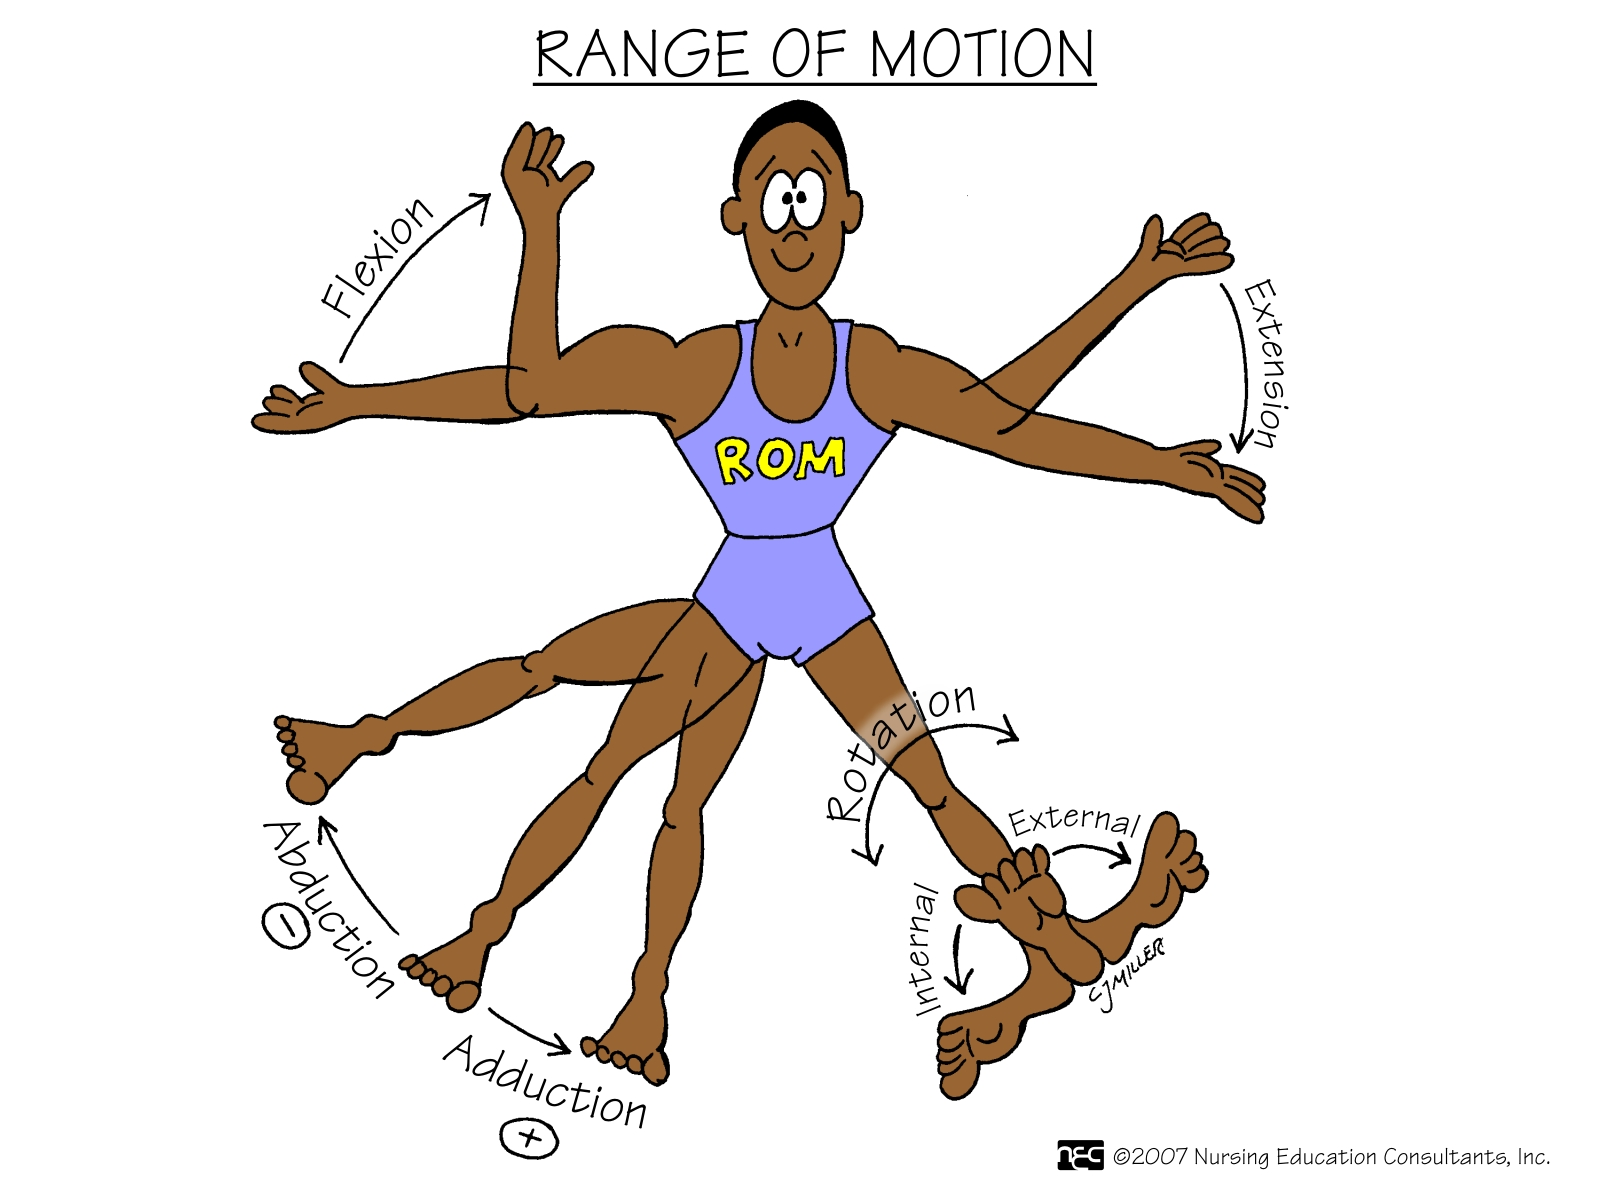
\includegraphics[scale=0.25]{fig/rangeofmotion.png}}  
  \caption{Range of Motion \cite{rangeofmotion}}
  \label{fig:rom-exemple}
\end{figure}

\par That's why we want to make a application which makes use of a camera to objectively 
calculate ROM in real-time and automatically produce a report that tracks progress over the course 
of several therapy sessions.

% O altă abordare pe care o folosim pentru a măsura progresul 
% mișcării pacientului, consta in masurarea distantei care o parcurg mainile 
% si picioarele pacientului. De exemplu daca pacientul face o sesiune 
% de exerciti dupa finalizarea sesiuni vom putea vedea un 
% raport cu dinstanta maini drepte si stangi , la fel si pentru picioare.
Another approach we use to measure the progress of patient movement is 
to measure the distance of the patient's hands and feet. For example, 
if the patient performs an exercise session after the session is completed we will 
be able to see a report with the right and left hands, as well as the legs.

% In aceasta lucrare vom incerca sa implementam doua prototipuri de aplicati,
%  una web si una mobile in 
% care vom trat cele doua abordari de urmarire a progresului descrise mai sus.
In this paper we will try to implement two prototypes of applications, 
a web application and a mobile application, 
in which we will address the two approaches to track progress described above.

\section{What is pose estimation?}

% Task-ul prin care se determina pozitia unui obiect intr-o imagine sau chiar pe un video 
% real-time cum este cazul din lucrearea de fata, se numeste pose estimation.
The task of determining the position of an object in an image 
or even a real-time video, as is the case in the present work, is called pose estimation.
Pose refers to the object’s position and orientation in the coordinate system.

% In industria de viziune pe calculator au aparut pentru prima data algoritmi 
% de pose estimation care au fost folositi in special in robotica, pentru a putea 
% programa un robot sa faca anumite task-uri cum ar fi sa mute anumite obiecte intr-un depozit.
In the computer vision industry, for the first time, pose estimation algorithms 
have been developed to be use especially in robotics, to schedule a robot to 
do certain tasks such as moving certain objects to a warehouse. \cite{book.computer.vision.2001}

The pose estimation problem can be solved in three ways:
\begin{itemize}
% Acesta metoda consta in identificare unui set de puncte de control asupra obiectului, de obicei se obtin pe baza unor caracteristici cum ar fi marginile
  \item Analytic or geometric method consists of identify a set of control points 
    on the object, usually obtained on the basis of features such as edges
% Algoritmul genetic constă în utilizarea pozițiilor ca reprezentare genetică și calcularea errori ca valoarea dintre proiecția punctelor de control a obiectului și imaginea bazată pe capacitatea de fitness
  \item Genetic algorithm consists in using positions as genetic representation and calculating errors
   as the value between the projection of the object control points and image based on fitness function.
 
 \item Learning-based  method uses a system based on artificial intelligence, usually convolutional neural network,
 in the next chapter we will describe how it works.
\end{itemize} 

%  În această lucrare am ales a treia metodă bazată pe inteligența artificială, considerată cea mai potrivită.
In this paper we choose the third method based on artificial intelligence, considered the most appropriate.

% Mai mult de atat noi incercam sa rulam acesti algoritmi pe in browser si pe dispozitive mobile, iar in capitolul 4 vom explica in amanunt aceste detali.
More than that, we try to run these algorithms on the browser and on mobile devices, 
 in Chapter 4 we will explain in details.

% In continuare vom prezenta  mai multe detali despre algoritmi inteligenti care invatat sa detecteze pozitia partilor corpului
Below we will present more details about intelligent algorithms that have learned to detect the position of body parts.